
%
% state - drupal mapping
%

\section{Drupal \& Mapping}
\label{chapter:drupal-mapping}

As the web, Drupal is a constantly evolving platform. The book ``Mapping with Drupal''\cite{Zzolo11mappingdrupal} by Alan Palazzolo and Thomas Turnbull was published in the end of 2011 and gives a throughout overview of available mapping modules for Drupal 7 by that time. Development obviously continued since then, so its a continuous exercise to keep up-to-date with recent technologies.

\subsection{Data storage}

The \textbf{Geofield}\footnote{\url{http://drupal.org/project/geofield}} module is stated to be the ``best choice for all but the simplest mapping applications''\cite[page 27]{Zzolo11mappingdrupal} in Drupal 7. By using the \textit{geoPHP library}\footnote{\url{https://github.com/phayes/geoPHP}} for geometry operations it allows to store location data in various formats as latitude/longitude, WKT. It integrates with various other mapping modules related to data input and storage in Drupal, as illustrated in figure \ref{fig:geofield}.

\begin{figure}[h]
  \begin{center}
    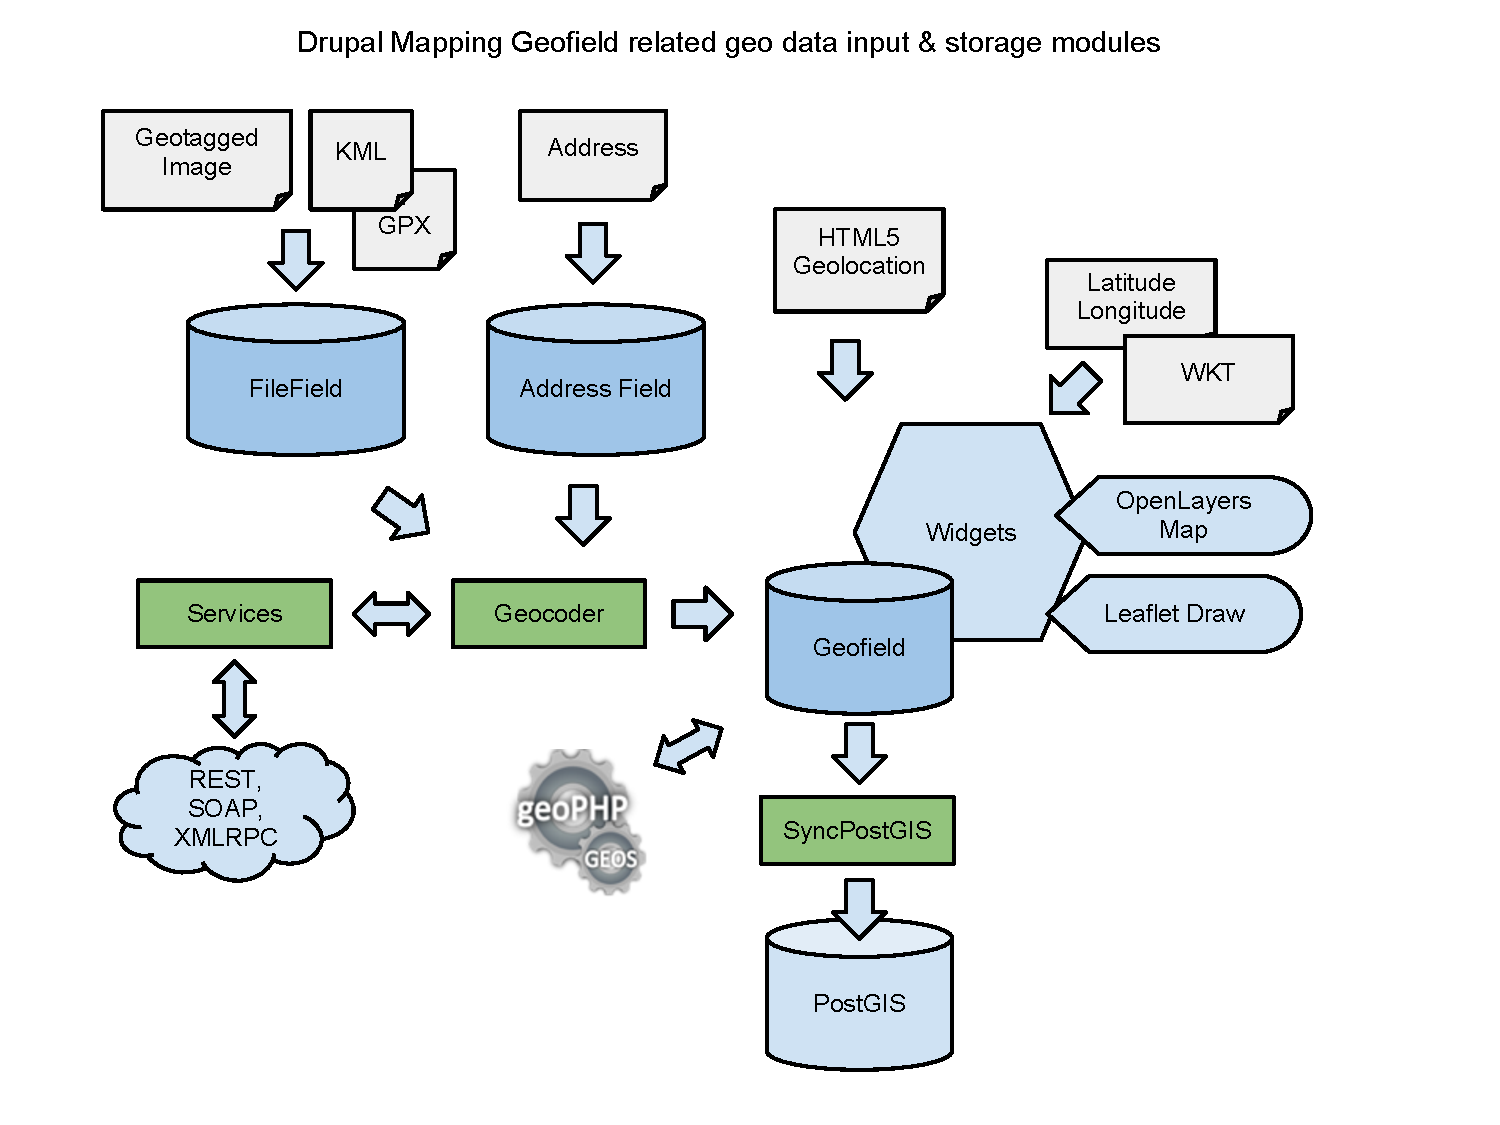
\includegraphics[width=1.2\textwidth]{figures/drupal_mapping_geofield.pdf}
    \caption{The Drupal Geofield module and related geo data input and storage modules.}
    \label{fig:geofield}
  \end{center}
\end{figure}

Besides the geofield module, the following modules are relevant to its main task of storing location data: 

\begin{itemize}

\item \textbf{PostGIS integration} is often requested when dealing with complex spatial data. A variety of modules and approaches exist for integration with PostGIS. The \textit{PostGIS} module\footnote{\url{http://drupal.org/project/postgis}} is similar to Geofield but relies on PostGIS for spatial operations and data storage. \textit{Sync PostGIS}\footnote{\url{http://drupal.org/project/sync_postgis}} allows to push geospatial data from a Drupal-internal storage as Geofield into PostGIS. Recently, a pluggable storage backend was added\footnote{\url{http://drupal.org/node/1728530}} to the Geofield module in order to allow integration with alternative databases. \textit{Geofield PostGIS}\footnote{\url{https://github.com/phayes/geofield_postgis}} therefore is a more integrated option for storing Geofield data in PostGIS.

\item \textbf{Solr integration} is another common approach when creating maps based on Drupal. \textit{Apache Solr search} is a fast open source search platform written in the Java programming language. There are two common modules for Solr integration in Drupal which both offer support for indexing spatial data: \textit{Search API}\footnote{\url{http://drupal.org/project/search_api}} and \textit{Apache Solr Search Integration}\footnote{\url{http://drupal.org/project/apachesolr}}.

\item The \textbf{Location}\footnote{\url{http://drupal.org/project/location}} module is another popular choice for storing spatial data in Drupal 7. As its architecture doesn't follow current Drupal conventions, its rather a monolithic system that provides a rich out-of-the-box experience but doesn't integrate that well with other modules like Geofield does~\cite{Zzolo11mappingdrupal}.

\end{itemize}

\subsection{Data presentation}

Being a content management system and framework, the second most important task for handling spatial data in Drupal is presenting it in various ways. Again, a variety of modules exists for querying and displaying geospatial data. Figure \ref{fig:drupal-mapping-display} illustrates how the query- and display-related Drupal mapping modules work together in a common use case.

A \textbf{mapping module} provides the basic integration a JavaScript mapping library with the Drupal internals. The most widely used mapping modules are the \textit{OpenLayers} module\footnote{\url{http://drupal.org/project/openlayers}} with 7,205 active installations on Drupal 7 by January 2012 and the GMap module\footnote{\url{http://drupal.org/project/gmap}} with 21,920. The Leaflet module\footnote{\url{http://drupal.org/project/leaflet}} only counts 496 active installations reported by drupal.org by that time, but has the advantage of being more lightweight than OpenLayers and is not bound to a single, commercial API as GMap.

\begin{figure}[h]
  \begin{center}
    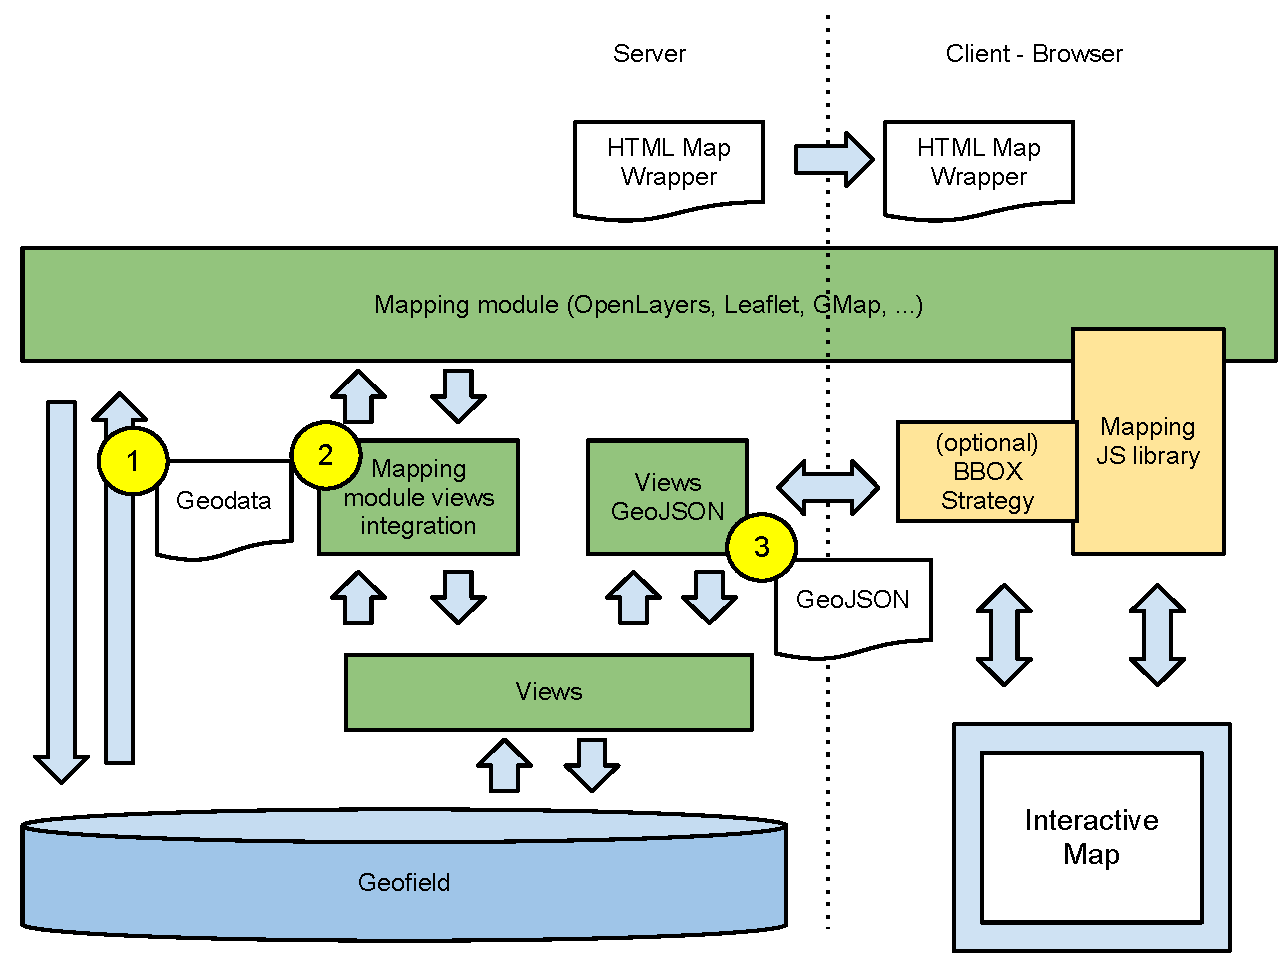
\includegraphics[width=1\textwidth]{figures/drupal_mapping_display.pdf}
    \caption{The prototypic work-flow of query and display-related Drupal mapping modules.}
    \label{fig:drupal-mapping-display}
  \end{center}
\end{figure}

The interaction with the spatial data provided by the Geofield module can be classified into three different scenario types, visualized by circles within figure \ref{fig:drupal-mapping-display}:

\begin{enumerate}

\item In the first scenario, the mapping module directly accesses data from Geofield. This approach is usually applied when displaying maps with single location items. The geodata retrieved from Geofield is then transferred to the client within the HTML response. On the client-side, the JavaScript mapping library takes care of visualizing the geodata.

\item In the second scenario, integration with the \textbf{Views} module is used to query a collection of data. Integrating with Views allows the mapping module to query a listing of locations from geofield, based user-defined parameters. Instead of returning single locations as in scenario one, the second therefore processes a collection of geodata values.

The Drupal \textit{Views} module\footnote{\url{http://drupal.org/project/views}} is the de-facto standard for creating listings of content of any kind. With 377,956 reported installations by January 2012 it is the most widely used module and it will be part of Drupal 8 core. This powerful tool allows site builders to configure database queries using an administration interface. In addition, the module provides formatting options for representing query results. In combination with extension modules the Views module allows to create lists, tables and many other formats.  

\item Scenario three allows for dynamically updating the map based on user interaction. In this case, the geospatial data is not delivered within the HTML response as in the previous approaches. The JavaScript library issues a separate request to the server using a \textbf{Bounding Box strategy}. The OpenLayers JavaScript library contains such a BBOX Strategy\footnote{\url{http://dev.openlayers.org/docs/files/OpenLayers/Strategy/BBOX-js.html}} and the \textit{Leaflet GeoJSON} module\footnote{\url{http://drupal.org/project/leaflet_geojson}} provides the same for the Leaflet library. The strategy essentially requests the geodata within the bounding box of the current viewport. On the server-side, the \textit{Views GeoJSON} module\footnote{\url{http://drupal.org/project/views_geojson}} translates the query and transforms the data returned by Views into a \textit{GeoJSON}\footnote{\url{http://www.geojson.org/}} feed in order to deliver it to the JavaScript mapping library on the client-side.

\end{enumerate}

Note that the exact implementation details vary between the used mapping modules.

\textbf{Solr integration} for querying and displaying geospatial data in Drupal is mainly provided by the integration of the modules with Views. In addition, for the \textit{Apache Solr Search Integration} module exists a \textit{apachesolr\_location} module\footnote{\url{http://drupal.org/project/apachesolr_location}} and a \textit{ApacheSolr Geo} sandbox project\footnote{\url{http://drupal.org/sandbox/pwolanin/1497066}}. For \textit{Search API} there is a \textit{Search API Location}\footnote{\url{http://drupal.org/project/search_api_location}} module.


